\chapter{Implementación y desarrollo} % Main chapter title

\label{Chapter3} % Change X to a consecutive number; for referencing this chapter elsewhere, use \ref{ChapterX}

Este capítulo expone el proceso técnico de implementación y desarrollo del sistema propuesto. En primer lugar, se describe la arquitectura de la solución, instancia en la que se definió la separación de responsabilidades entre la aplicación base y el SDK nativo denominado Aurum. A continuación, se detalla el modelo de datos estructurado que se diseñó para encapsular las intenciones y entidades extraídas de los comandos de voz. Finalmente, se explican los componentes del código fuente del prototipo.

\definecolor{mygreen}{rgb}{0,0.6,0}
\definecolor{mygray}{rgb}{0.5,0.5,0.5}
\definecolor{mymauve}{rgb}{0.58,0,0.82}

%%%%%%%%%%%%%%%%%%%%%%%%%%%%%%%%%%%%%%%%%%%%%%%%%%%%%%%%%%%%%%%%%%%%%%%%%%%%%
% parámetros para configurar el formato del código en los entornos lstlisting
%%%%%%%%%%%%%%%%%%%%%%%%%%%%%%%%%%%%%%%%%%%%%%%%%%%%%%%%%%%%%%%%%%%%%%%%%%%%%
\lstset{ %
  backgroundcolor=\color{white},   % choose the background color; you must add \usepackage{color} or \usepackage{xcolor}
  basicstyle=\footnotesize,        % the size of the fonts that are used for the code
  breakatwhitespace=false,         % sets if automatic breaks should only happen at whitespace
  breaklines=true,                 % sets automatic line breaking
  captionpos=b,                    % sets the caption-position to bottom
  commentstyle=\color{mygreen},    % comment style
  deletekeywords={...},            % if you want to delete keywords from the given language
  %escapeinside={\%*}{*)},          % if you want to add LaTeX within your code
  %extendedchars=true,              % lets you use non-ASCII characters; for 8-bits encodings only, does not work with UTF-8
  %frame=single,	                % adds a frame around the code
  keepspaces=true,                 % keeps spaces in text, useful for keeping indentation of code (possibly needs columns=flexible)
  keywordstyle=\color{blue},       % keyword style
  language=[ANSI]C,                % the language of the code
  %otherkeywords={*,...},           % if you want to add more keywords to the set
  numbers=left,                    % where to put the line-numbers; possible values are (none, left, right)
  numbersep=5pt,                   % how far the line-numbers are from the code
  numberstyle=\tiny\color{mygray}, % the style that is used for the line-numbers
  rulecolor=\color{black},         % if not set, the frame-color may be changed on line-breaks within not-black text (e.g. comments (green here))
  showspaces=false,                % show spaces everywhere adding particular underscores; it overrides 'showstringspaces'
  showstringspaces=false,          % underline spaces within strings only
  showtabs=false,                  % show tabs within strings adding particular underscores
  stepnumber=1,                    % the step between two line-numbers. If it's 1, each line will be numbered
  stringstyle=\color{mymauve},     % string literal style
  tabsize=2,	                   % sets default tabsize to 2 spaces
  title=\lstname,                  % show the filename of files included with \lstinputlisting; also try caption instead of title
  morecomment=[s]{/*}{*/}
}


%----------------------------------------------------------------------------------------
%	SECTION 1
%----------------------------------------------------------------------------------------

\section{Arquitectura del sistema}

A continuación, se detallan cada una de las fases técnicas atravesadas para la elaboración de este trabajo.

\begin{itemize}
	\item Comprensión del negocio: esta fase inicial constituye el pilar fundamental del trabajo, dado que define el puente entre la necesidad de accesibilidad del usuario y las exigencias transaccionales del sistema bancario. El problema central del negocio radica en las barreras de usabilidad que las interfaces táctiles tradicionales imponen a personas con discapacidades visuales o motoras. La solución propuesta es habilitar un canal conversacional.
	
Desde la perspectiva del sistema, la comprensión del negocio se traduce en el desafío algorítmico de transformar lenguaje natural, inherentemente ambiguo y desestructurado, en formatos estructurados y accionables que el core bancario pueda procesar de manera segura. Por ejemplo, una expresión coloquial como "transferile cinco mil pesos a mamá`` carece de utilidad directa para una base de datos financiera. El objetivo del negocio exige que el pipeline de IA sea capaz de capturar esta emisión acústica y extraer inequívocamente una intención principal (Clasificación de Intención: TRANSFERENCIA) y los parámetros o entidades asociadas (Reconocimiento de Entidades Nombradas: MONTO: 5000, MONEDA: ARS, DESTINATARIO: mamá). Solamente al mapear el habla hacia este diccionario de datos estructurado (típicamente en formato JSON o estructuras nativas de Swift), el sistema móvil puede invocar la lógica de negocio correspondiente, lo que garantiza una operación determinista, libre de ambigüedades y sin fricción para el usuario.

	\item Comprensión de los datos: una vez definido el objetivo de extraer intenciones y entidades transaccionales, esta fase se centra en identificar la naturaleza y los requerimientos de la información necesaria para entrenar el modelo. En el contexto de la banca móvil, los datos reales de los usuarios están protegidos por estrictas normativas de privacidad y secreto bancario. Al tratarse de una prueba de concepto y ante la ausencia de un registro histórico de comandos de voz accionados por usuarios, se determinó la necesidad de construir un conjunto de datos (\textit{dataset}) sintético. En esta etapa se analizó la morfología del lenguaje coloquial rioplatense aplicado a finanzas, identifica sinónimos de acciones (transferir, enviar, pasar plata), variaciones en la expresión de montos (números cardinales, fracciones) y formas comunes de nombrar contactos.
	
	\item Evaluación: esta fase contrastó los resultados empíricos del modelo contra los criterios de éxito definidos al inicio del trabajo. A nivel algorítmico, se midió el desempeño predictivo que utiliza un conjunto de prueba aislado, que calcula métricas de Accuracy para la clasificación de intenciones, así como Precision, Recall y F1-Score para el reconocimiento de entidades. A nivel de negocio e integración, la evaluación trascendió las métricas puramente matemáticas para incorporar pruebas de usabilidad en el entorno simulado de iOS, mide la latencia de la inferencia local y la tasa de éxito de la tarea integral. Esto permitió verificar que la extracción estructurada lograra, en efecto, completar el flujo de la aplicación sin errores perjudiciales para la experiencia del usuario.
	
	\item Despliegue: en un proyecto de analítica tradicional, el despliegue suele implicar la exposición del modelo a través de una API en un servidor en la nube. Sin embargo, en esta prueba de concepto, la fase de despliegue se redefinió para cumplir con el requisito innegociable de máxima privacidad. El despliegue consistió en la conversión de los modelos entrenados al formato \lstinline|.mlpackage|, su integración directa en el código fuente del proyecto en Xcode, y su invocación local mediante el framework Core ML. De esta manera, el modelo se "desplegó" \ encapsulado dentro del propio binario de la aplicación iOS, se garatiza que el pipeline de transformación de voz a texto (vía AVFoundation y Speech) y la posterior comprensión del lenguaje natural se ejecuten de manera estrictamente local en el dispositivo del usuario final.
	
\end{itemize}


El diseño arquitectónico de la presente prueba de concepto se fundamenta en el paradigma de computación Edge AI, trasladando la carga computacional de los algoritmos de inteligencia artificial directamente al dispositivo móvil del usuario. Esta decisión estratégica persigue un doble objetivo metodológico y normativo: por un lado, minimizar la latencia inherente a las comunicaciones de red corporativas y, por otro, garantizar un entorno de privacidad por diseño. Al ejecutar los modelos a través del \textit{framework} Core ML, los flujos de audio y las transcripciones de índole financiera no abandonan en ningún momento el entorno físico del hardware de Apple, lo que mitiga drásticamente los vectores de ataque asociados a la interceptación de datos en tránsito o al almacenamiento temporal en servidores de terceros.
Para asegurar la escalabilidad, la modularidad y la mantenibilidad del código, el sistema fue concebido bajo el principio de separación de responsabilidades. La solución se estructura en dos grandes bloques funcionales e independientes: la aplicación base anfitriona y el SDK nativo Aurum \citep{apple2026frameworks}. Es imperativo establecer una restricción arquitectónica crítica que define los límites de esta integración: el proyecto no incluye, bajo ninguna circunstancia, algoritmos de validación biométrica de voz. La autenticación de la identidad del cliente, el manejo de tokens de sesión y las medidas de seguridad perimetral recaen, de manera exclusiva y excluyente, sobre la aplicación móvil del banco. En este modelo topológico, el SDK Aurum opera bajo la premisa de confianza de que es invocado dentro de un contexto transaccional previamente segurizado por la entidad financiera, lo que hace adoptar el dominio de responsabilidad estrictamente a la captura acústica, la transcripción y la extracción semántica de intenciones y entidades.

En la figura \ref{fig:diagComp} se presenta el diagrama de componentes.

\begin{figure}[htpb]
\centering 
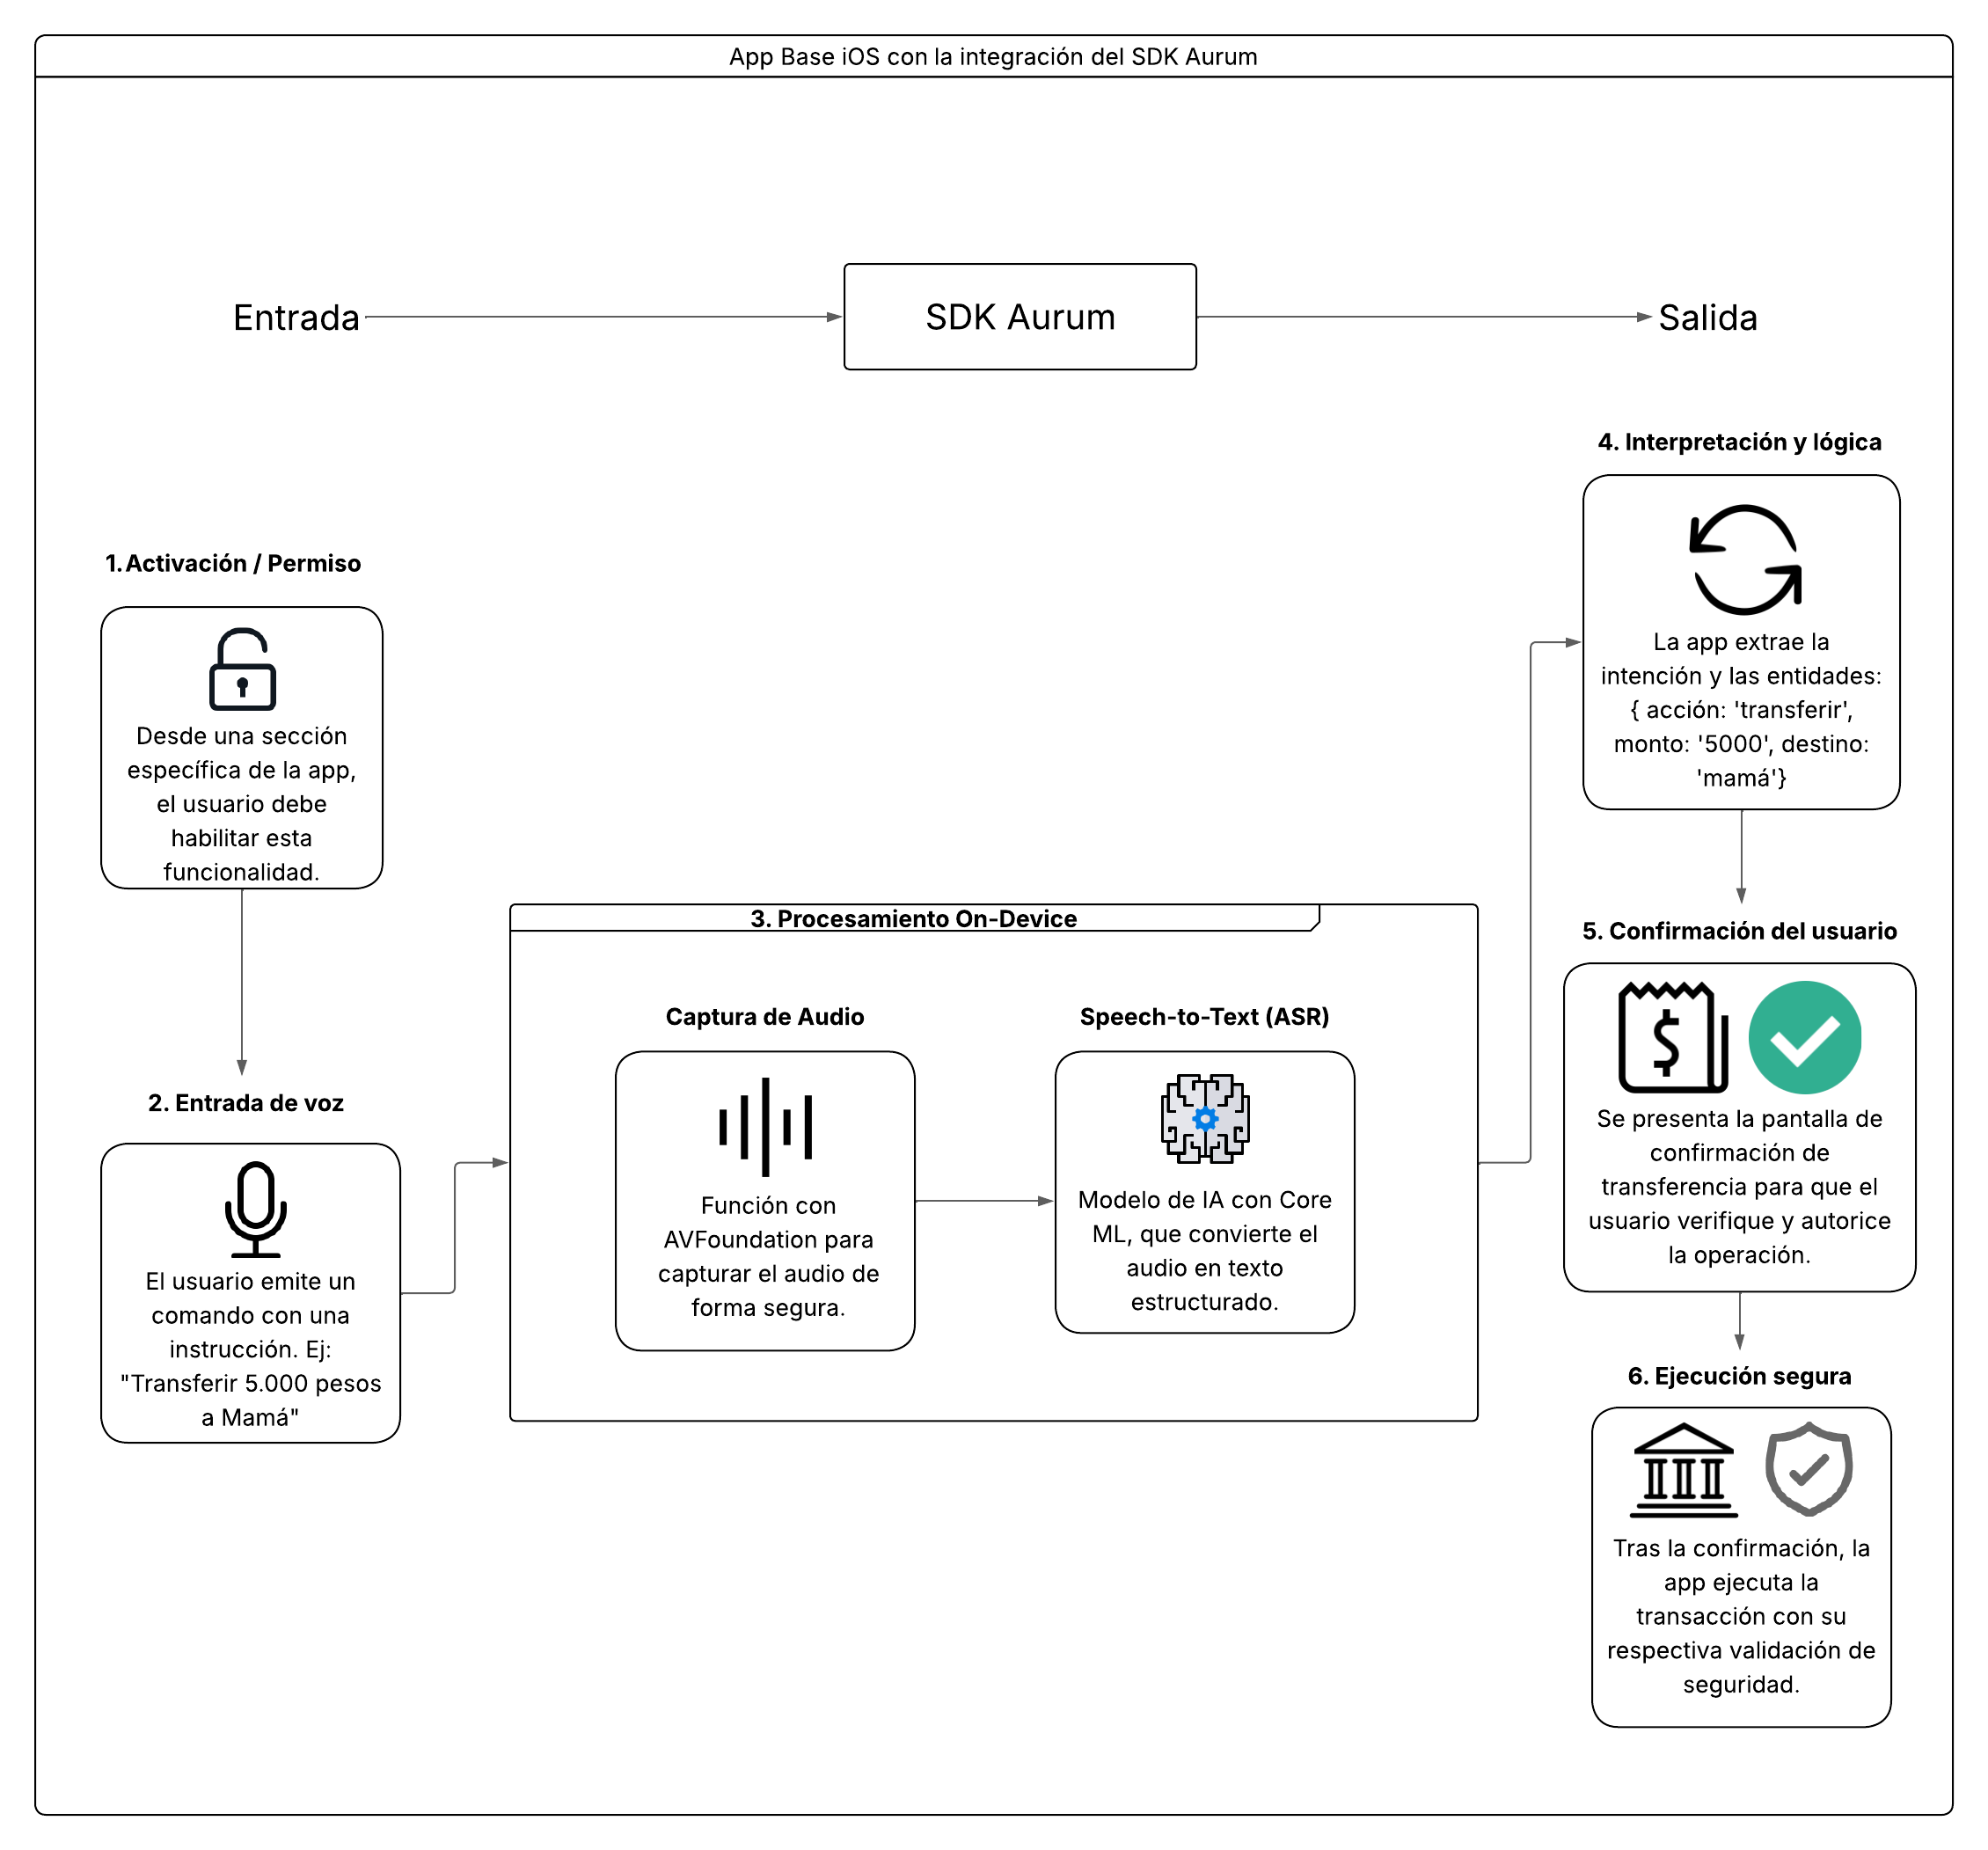
\includegraphics[width=1.0\textwidth]{./Figures/diagrama-de-componentes.png}
\caption{Diagrama de arquitectura de componentes que conforman la prueba de concepto.}
\label{fig:diagComp}
\end{figure}

El ciclo de vida de una transacción impulsada por voz atraviesa un pipeline determinista que fluye secuencialmente a través de las capas de la arquitectura descrita. El proceso de ingesta de datos se desencadena en la aplicación base cuando el usuario, luego de superar los controles de acceso convencionales del banco, interactúa con el disparador de la interfaz gráfica (botón de dictado). En ese instante, la aplicación anfitriona invoca la API pública del SDK Aurum, transfiriéndole el control del hilo de ejecución de audio. El SDK inicializa una sesión de captura de alto rendimiento mediante el framework AVFoundation, configurando el entorno acústico adecuado para aislar la frecuencia de la voz humana.
Una vez digitalizada la señal de audio, el motor interno del SDK emplea las capacidades de transcripción fuera de línea (offline) provistas por las librerías nativas de iOS para ejecutar el reconocimiento automático de habla, esto convierte el espectrograma en una cadena de texto cruda. Acto seguido, este texto es sometido a técnicas de normalización morfológica y es inyectado en el motor de comprensión del lenguaje natural. En esta fase de inferencia, la transcripción es procesada localmente por los modelos vectoriales preentrenados y cuantizados alojados en Core ML. Dichos modelos resuelven algorítmicamente el problema de clasificación de la intención del usuario y proceden al etiquetado posicional para extraer las variables nominales del comando.
El flujo de información concluye cuando la salida matricial de las redes neuronales es traducida por el SDK en un payload \citep{sommerville2015software} de datos estructurado y fuertemente tipado. Este artefacto resultante, que encapsula inequívocamente la acción solicitada, la magnitud numérica del monto, el tipo de divisa y la identidad del beneficiario, es retornado de manera asíncrona a la aplicación anfitriona a través de patrones de delegación (\textit{Delegates o Closures})\citep{apple2026swiftlanguage}. A partir de la entrega de este objeto estructurado, el SDK Aurum finaliza su intervención y cede nuevamente el control a la aplicación base que asume la responsabilidad de mapear el payload contra su modelo de datos transaccional, renderizar la interfaz de validación final ante el usuario y proceder con la comunicación cifrada hacia el core bancario.

En la figura \ref{fig:pipelineVoz} se muestra el flujo del pipeline (ciclo de vida de una transacción por voz).

\begin{figure}[htpb]
\centering 
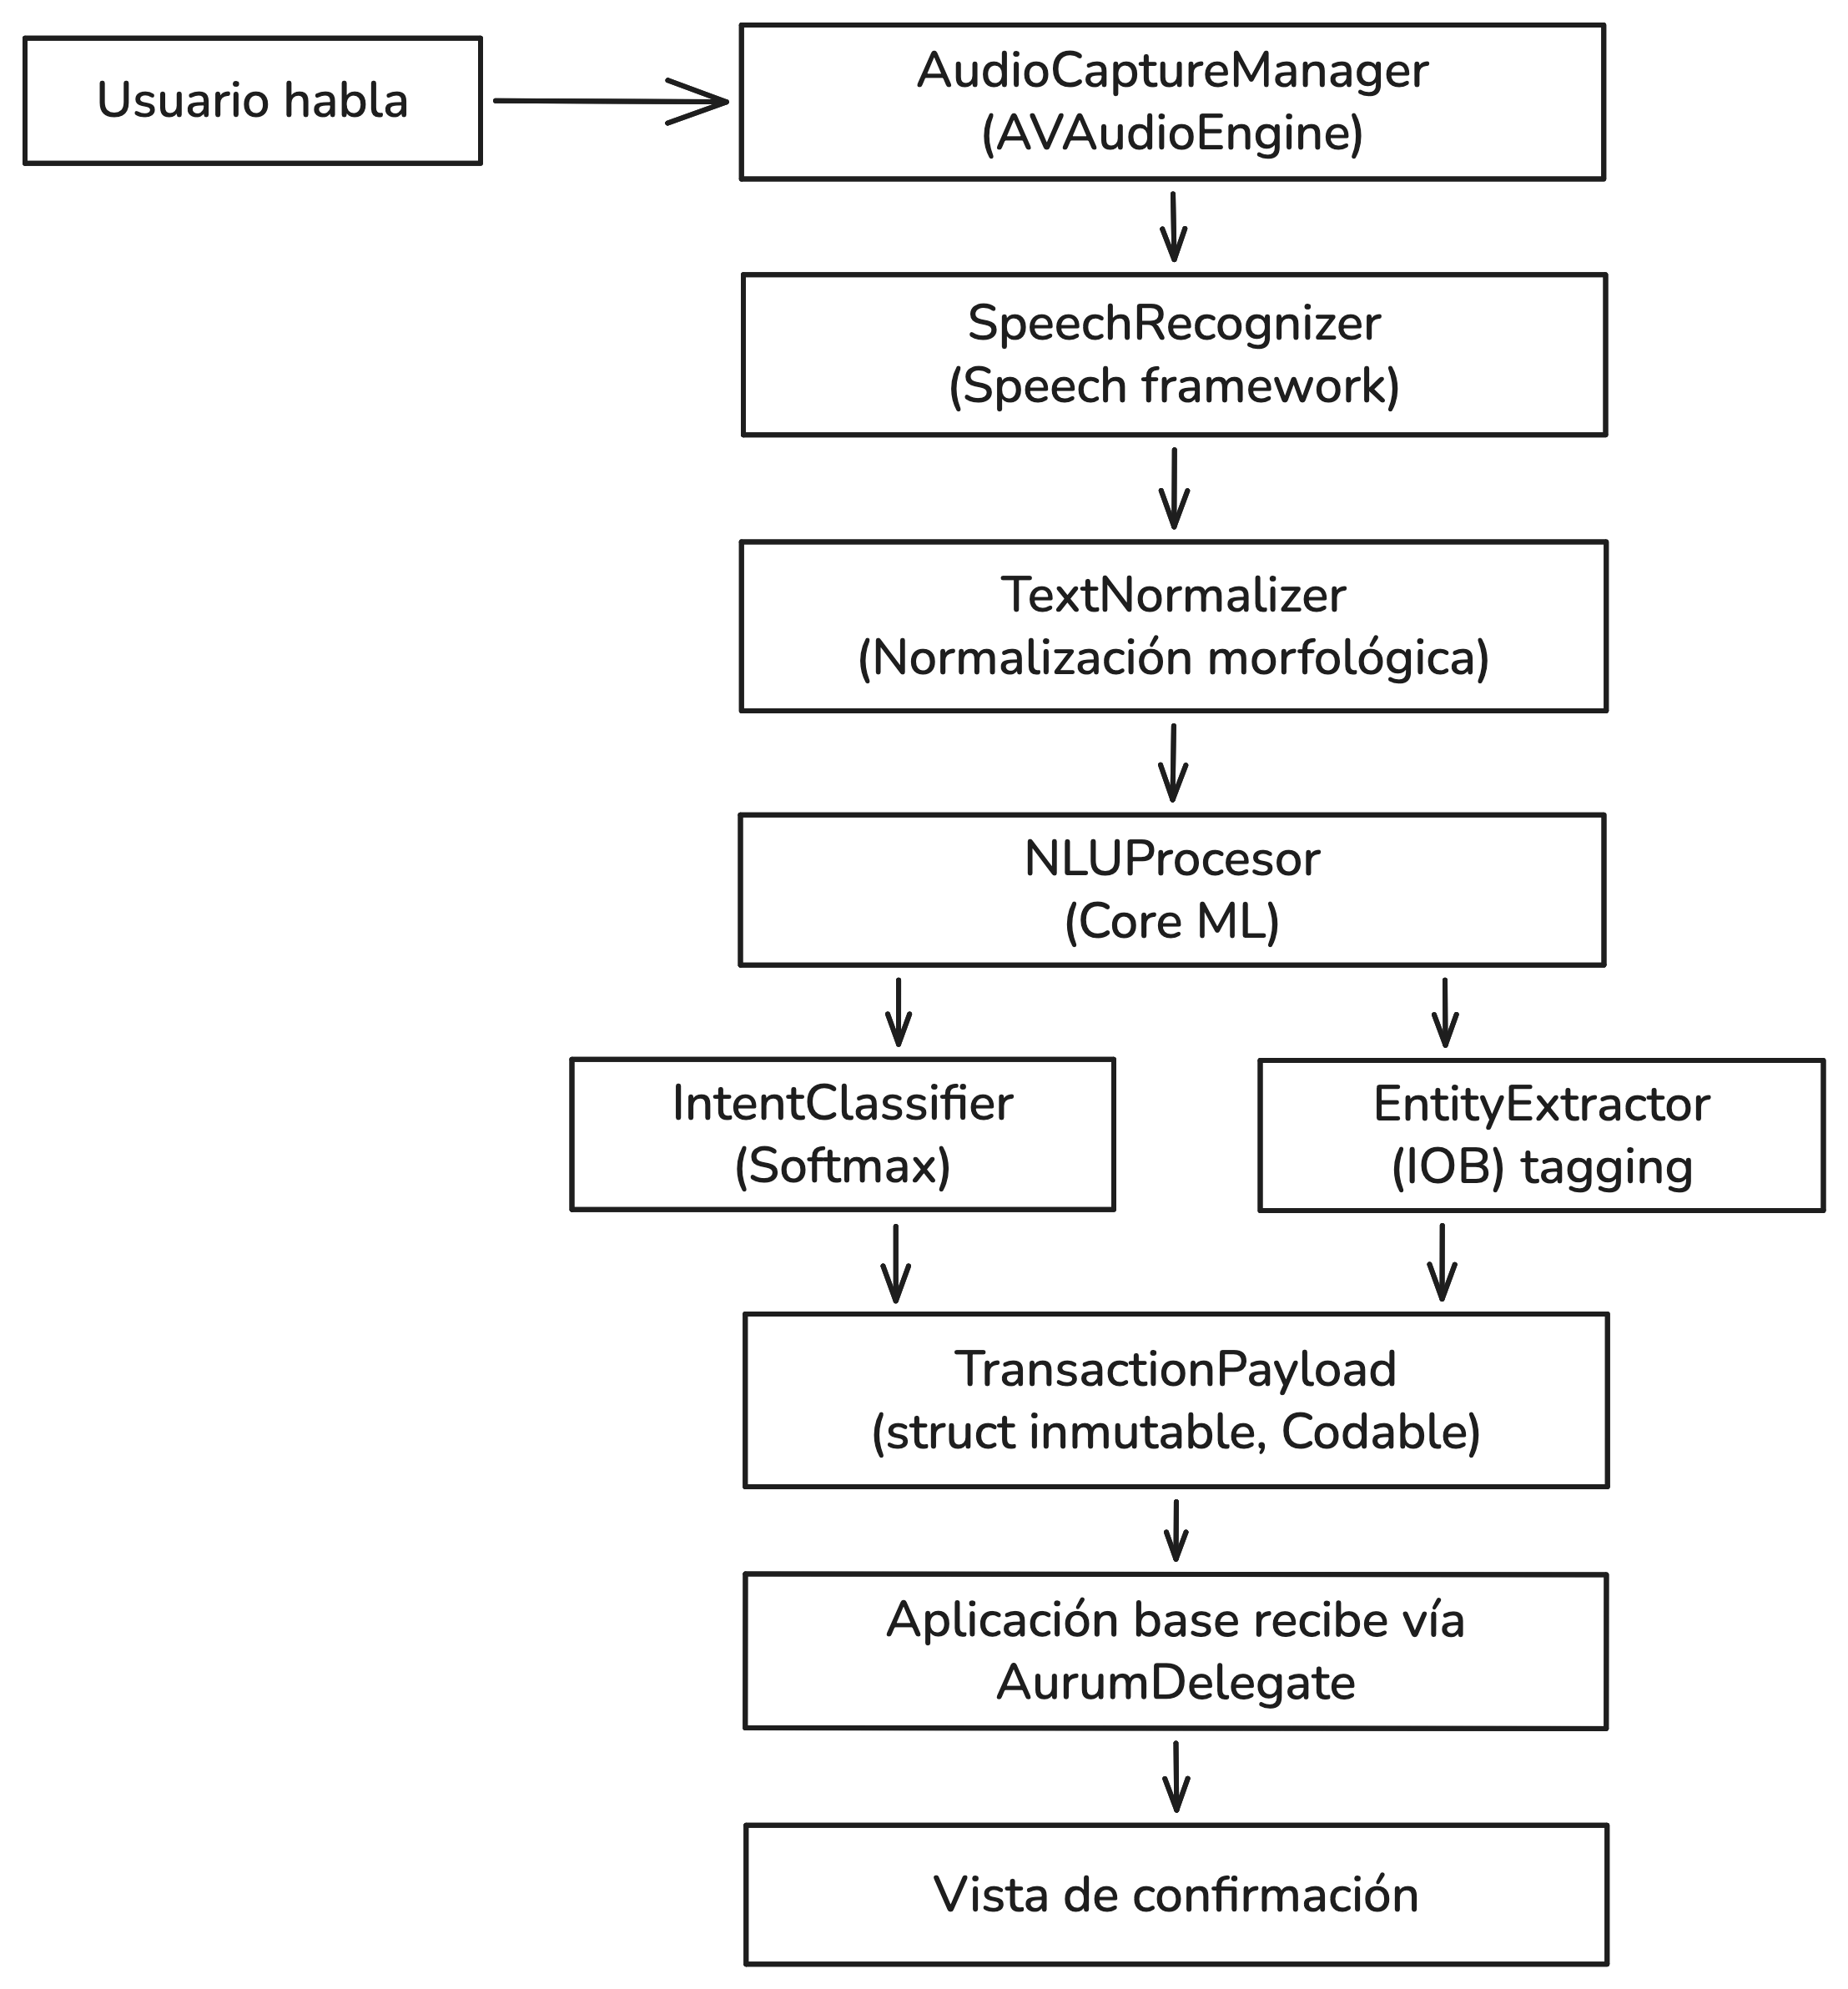
\includegraphics[width=1.0\textwidth]{./Figures/pipeline-transaccion.png}
\vspace{0.5cm} 
\caption{Flujo de pipeline de una transacción realizada por voz.}
\label{fig:pipelineVoz}
\end{figure}

\section{Tratamiento y preparación de datos}

El desarrollo de modelos de procesamiento de lenguaje natural aplicados a dominios de misión crítica, como el sector bancario, enfrenta el desafío inherente del acceso a la información, conocido como el problema de arranque en frío \ (\textit{cold start}). Las estrictas normativas de privacidad y el secreto bancario imposibilitan el uso de corpus conversacionales de clientes reales sin someterlos previamente a procesos de anonimización complejos y costosos. Adicionalmente, al tratarse de una prueba de concepto que introduce un canal de interacción inédito en el entorno simulado de la aplicación móvil, no existe telemetría histórica ni registros acústicos o textuales previos de comandos transaccionales.
Ante esta restricción, se determinó como exigencia metodológica la generación de un conjunto de datos sintéticos (\textit{mock data}). La construcción de un corpus artificial permite no solo superar la ausencia de datos iniciales, sino también ejercer un control riguroso sobre la distribución probabilística de las clases (intenciones) y garantizar una cobertura exhaustiva de los casos límite (\textit{edge cases}) de las entidades. Este enfoque metodológico aísla el desarrollo algorítmico de los riesgos de privacidad y provee un entorno determinista, fundamental para iterar la arquitectura de la red neuronal durante las primeras fases de evaluación.


\subsection {Creación de plantillas de comandos y aumentación de datos}

La síntesis del corpus de entrenamiento se estructuró a partir de la definición de plantillas (\textit{templates}) gramaticales. Estas plantillas modelan lógicamente las posibles estructuras sintácticas que un usuario emplearía para interactuar con el sistema bancario y se abstraen los valores concretos, tales como: [ACCIÓN] [MONTO] [MONEDA] a [DESTINATARIO].
Una vez consolidadas las estructuras base, se implementaron técnicas de aumentación de datos (\textit{data augmentation}) para inyectar la variabilidad inherente al lenguaje natural \cite{feng2021survey}.

La transición entre el entorno probabilístico inherente a los modelos de machine learning y el rigor determinista exigido por los sistemas financieros requiere de una capa de abstracción robusta. Para resolver este paradigma, se estructuraron los datos resultantes de la inferencia algorítmica utilizando estructuras de valor \textit{struct} en Swift  \citep{apple2026swiftlanguage}. El uso de \textit{structs} garantizó la inmutabilidad de la información una vez extraída y procesada, esto prevee alteraciones accidentales de las variables en la memoria durante el ciclo de vida de la transacción.
Para la serialización de este modelo, se adoptó el protocolo Codable nativo de Apple \citep{apple2026codable}. Esta decisión arquitectónica se justificó en la necesidad de estandarizar la comunicación entre el SDK y la aplicación base, así el objeto Swift generado en memoria puede ser codificado y decodificado de manera nativa hacia formatos universales de intercambio de datos, como JSON \citep{rfc8259json}, sin depender de librerías de terceros.

\subsection{Modelo de datos}

El diseño del payload (o carga útil) que el modelo de etiquetado de secuencias (NER) y el clasificador de intenciones devolvieron al sistema se consolidó en una única entidad semántica. Durante el desarrollo, se definieron campos fuertemente tipados para encapsular de manera exacta las variables transaccionales críticas:

\begin{itemize}
	\item Intención: representa la acción directiva inferida del comando verbal (por ejemplo, iniciar una transferencia). Se estructuró como el eje central que define el ruteo posterior dentro de la aplicación.
	\item Monto: se tipificó mediante el uso de datos de punto flotante de doble precisión (\textit{Double}) \citep{apple2026swiftlanguage}, esto permite la representación matemática de la magnitud monetaria extraída de la transcripción fonética.
	\item Moneda: se modeló utilizando enumeraciones (\textit{Enum}) con tipos crudos de cadena de texto (\textit{String raw values}) \citep{apple2026swiftlanguage}. Esto restringió el dominio de la divisa a valores finitos y normalizados bajo estándares internacionales (ej. ARS o USD), eliminando la ambigüedad de sinónimos coloquiales capturados por el motor NLU, como "pesos", "lucas"\ o "dólares".
	\item Destinatario: se definió como una cadena de caracteres cruda (\textit{String}) \citep{apple2026swiftlanguage} que encapsula la identidad nominal del beneficiario de la operación, dejando el valor preparado para ser contrastado posteriormente contra la agenda de contactos o base de alias validada del banco.
\end{itemize}

Este enfoque de modelado determinista cumple una función vital en la arquitectura de integración del sistema. Al transformar una emisión acústica originalmente desestructurada en un objeto Swift predecible y validado a nivel de compilador, se abstrajo a la aplicación anfitriona de toda la complejidad inherente al procesamiento de lenguaje natural. En consecuencia, la integración con los servicios de backend del banco se facilita de manera significativa: la aplicación móvil anfitriona consume un payload limpio, cuya estructura es análoga a la que generaría una interfaz táctil tradicional basada en formularios. Esto habilita a la aplicación base a tomar dichas variables tipadas e inyectarlas de manera directa en los constructores de sus peticiones de red seguras, esto mantendría intacta la lógica de consumo de los endpoints transaccionales de la institución.

\section{Desarrollo del SDK (Aurum)}

El desarrollo de Aurum se abordó bajo el paradigma de la programación orientada a componentes y se materializó como un \textit{framework} dinámico reutilizable dentro del ecosistema de Apple. El propósito fundamental de este encapsulamiento fue abstraer la complejidad algorítmica inherente al procesamiento de señales acústicas y a la inferencia de modelos de \textit{machine learning}, proporcionando a la aplicación bancaria anfitriona una interfaz programática mínima que oculta la totalidad de las operaciones internas. Al aislar el \textit{pipeline} de inteligencia artificial en un módulo independiente, se garantizó la cohesión del código, se facilitó su distribución y mantenimiento futuro, y se evitó la contaminación de la lógica de negocio y de la interfaz de usuario de la aplicación consumidora.

La arquitectura interna del SDK se organiza en cinco componentes especializados, cada uno con una responsabilidad bien delimitada, que se ejecutan de forma secuencial y coordinada bajo la orquestación de una clase fachada principal. La tabla~\ref{tab:componentes-sdk} presenta un resumen de estos componentes y sus dependencias de frameworks nativos de Apple.

Las secciones siguientes describen el diseño e implementación de cada componente, así como la API pública expuesta a la aplicación consumidora.

\begin{table}[htbp]
\centering
% Cambiamos la última 'l' por 'p{4.5cm}' (puedes ajustar el 4.5cm según necesites)
\begin{tabular}{@{} p{3.0cm} p{3.0cm} p{2.5cm} p{4.5cm} @{}}
\toprule
\textbf{Componente} & \textbf{Clase} & \textbf{Framework} & \textbf{Responsabilidad} \\
\midrule
Fachada principal
    & \lstinline|AurumEngine|
    & ---
    & Orquestación del pipeline \\
Captura de audio
    & \lstinline|AudioCaptureManager|
    & AVFoundation
    & Configuración de sesión y captura de buffers \\
Reconocimiento de voz
    & \lstinline|SpeechRecognizer|
    & Speech
    & Transcripción \textit{on-device} \\
Normalización de texto
    & \lstinline|TextNormalizer|
    & Foundation
    & Conversión léxica y numérica \\
Procesamiento NLU
    & \lstinline|NLUProcessor|
    & \lstinline|NaturalLanguage, CoreML|
    & Clasificación de intención y extracción de entidades \\
\bottomrule
\end{tabular}
\caption{Componentes del SDK Aurum y sus dependencias de frameworks nativos.}
\label{tab:componentes-sdk}
\end{table}


\subsection{Clase fachada: \texttt{AurumEngine}}

Para orquestar la ejecución secuencial de las etapas de procesamiento, se implementó la clase \texttt{AurumEngine} siguiendo el patrón de diseño
\textit{Facade} \citep{gamma1994design}. Esta clase constituye el único punto de entrada público del SDK y su responsabilidad es coordinar el ciclo de vida integral de la transacción de voz: desde la activación del micrófono hasta la entrega del \texttt{TransactionPayload} resultante.

Internamente, \texttt{AurumEngine} mantiene referencias privadas a los cuatro componentes de procesamiento y los instancia durante la fase de configuración. La API pública expone únicamente tres métodos de control:

\begin{lstlisting}[caption={API pública de \texttt{AurumEngine}.},label={lst:aurum-engine}]
public class AurumEngine {

    public weak var delegate: AurumDelegate?

    private let audioManager = AudioCaptureManager()
    private let speechRecognizer = SpeechRecognizer()
    private let textNormalizer = TextNormalizer()
    private let nluProcessor = NLUProcessor()

    /// Precarga los modelos Core ML desde el bundle de la app.
    public func configure(bundle: Bundle) {
        nluProcessor.loadModels(from: bundle)
    }

    /// Inicia la captura de audio y el reconocimiento de voz.
    public func startListening() { /* ... */ }

    /// Detiene la captura y fuerza el procesamiento del texto acumulado.
    public func stopListening() { /* ... */ }

    /// Cancela la operacion en curso y libera recursos.
    public func cancelListening() { /* ... */ }
}
\end{lstlisting}


El método \texttt{configure(bundle:)} recibe el \texttt{Bundle} de la aplicación anfitriona para localizar los archivos \texttt{.mlmodelc} compilados
(\texttt{IntentClassifier} y \texttt{EntityExtractor}) e instanciar los objetos \texttt{NLModel} correspondientes. Esta precarga se ejecuta una única vez
durante el inicio de la aplicación y permite que las inferencias posteriores se resuelvan con latencia mínima, evitando el costo de carga en caliente
(\textit{cold start}) durante la interacción de voz.


\subsection{Captura de audio: \texttt{AudioCaptureManager}}

El primer eslabón del pipeline es la gestión del hardware de audio del dispositivo. El componente \texttt{AudioCaptureManager} encapsula la
interacción con los frameworks \texttt{AVAudioSession} y \texttt{AVAudioEngine} de Apple, y resuelve tres tareas técnicas:

\begin{enumerate}
    \item Solicitud de permisos: la primera invocación verifica el estado de autorización del micrófono mediante
    \texttt{AVAudioSession.recordPermission}. Si el permiso no fue concedido previamente, dispara la solicitud nativa del sistema operativo. En caso de
    denegación, el componente reporta un error tipado (\texttt{AurumError.microphonePermissionDenied}) sin intentar activar la
    captura.

    \item Configuración de la sesión de audio: se establece la categoría \texttt{.playAnd\linebreak Record} con modo \texttt{.measurement}. La
    categoría \texttt{.playAndRecord} permite la entrada y salida simultánea de audio (necesaria para dispositivos con altavoz activo), mientras que el modo \texttt{.measurement} desactiva los filtros de ecualización y cancelación de ruido del sistema, proporcionando una señal de audio cruda óptima para
    el reconocedor de voz.

    \item Instalación del \textit{tap} de audio: se accede al nodo de  entrada (\texttt{inputNode}) del \texttt{AVAudioEngine} y se instala un
    \textit{tap} que captura \textit{buffers} de audio en formato PCM a la frecuencia de muestreo nativa del micrófono (típicamente 44.1~kHz o
    48~kHz). Estos \textit{buffers} se canalizan al componente \texttt{Speech\linebreak Recognizer} mediante un cierre (\textit{closure}).
\end{enumerate}

\begin{lstlisting}[caption={Configuración de la sesión de audio y captura de \textit{buffers}.},label={lst:audio-capture}]
func startCapture(onBuffer: @escaping (AVAudioPCMBuffer) -> Void) throws {
    let session = AVAudioSession.sharedInstance()
    try session.setCategory(.playAndRecord, mode: .measurement,
                            options: [.defaultToSpeaker])
    try session.setActive(true)

    let inputNode = audioEngine.inputNode
    let format = inputNode.outputFormat(forBus: 0)

    inputNode.installTap(onBus: 0, bufferSize: 1024, format: format)
    { buffer, _ in
        onBuffer(buffer)
    }

    audioEngine.prepare()
    try audioEngine.start()
}
\end{lstlisting}

La detención de la captura (\texttt{stopCapture()}) remueve el \textit{tap}, detiene el \texttt{AVAudioEngine} y desactiva la sesión de audio, liberando el
hardware del micrófono para que otras aplicaciones puedan utilizarlo.

\subsection{Reconocimiento de voz: \texttt{SpeechRecognizer}} 

El componente \texttt{SpeechRecognizer} integra el \textit{framework} nativo \texttt{Speech} \cite{apple2026speech} para ejecutar la transcripción de voz a texto. Su diseño responde a dos requisitos fundamentales del sistema: el soporte para español rioplatense y la garantía de procesamiento exclusivamente local.

La instanciación del reconocedor se realiza con el \textit{locale} específico \texttt{es-AR} (español de Argentina), lo que activa el modelo acústico y el
modelo de lenguaje optimizados para las particularidades fonéticas y léxicas del habla rioplatense:

\begin{lstlisting}[caption={Configuración del reconocedor de voz con procesamiento \textit{on-device}.},label={lst:speech-recognizer}]
private let recognizer = SFSpeechRecognizer(
    locale: Locale(identifier: "es-AR")
)

func startRecognition(onPartial: @escaping (String) -> Void,
                      onFinal: @escaping (String) -> Void) {
    let request = SFSpeechAudioBufferRecognitionRequest()

    // Forzar procesamiento local: ningun audio sale del dispositivo
    request.requiresOnDeviceRecognition = true

    // Sugerencias contextuales para el dominio financiero
    request.contextualStrings = [
        "transferir", "transferencia", "enviar", "mandar",
        "consultar", "saldo", "cancelar", "anular",
        "pesos", "dolares", "lucas", "verdes", "mangos"
    ]

    recognizer?.recognitionTask(with: request) { result, error in
        guard let result = result else { return }
        let text = result.bestTranscription.formattedString
        if result.isFinal {
            onFinal(text)
        } else {
            onPartial(text)
        }
    }
}
\end{lstlisting}


La propiedad \texttt{requiresOnDeviceRecognition = true} es la piedra angular de la estrategia de privacidad del sistema. Esta configuración instruye al
\textit{Speech Framework} a utilizar exclusivamente el modelo de reconocimiento descargado localmente en el dispositivo, bloqueando cualquier transmisión de paquetes de audio a los servidores de Apple. Si el modelo local no se encuentra disponible (por ejemplo, porque el usuario no descargó el paquete de idioma texttt{es-AR} para uso sin conexión), el reconocedor reporta un error en lugar de recurrir silenciosamente al procesamiento en la nube.

La propiedad \texttt{contextualStrings} proporciona al motor de reconocimiento un vocabulario de refuerzo específico del dominio financiero. Al incluir
términos como ``transferencia'', ``saldo'' o ``lucas'', se incrementa la probabilidad de que el reconocedor transcriba correctamente estas palabras
frente a alternativas fonéticamente similares pero semánticamente irrelevantes. Este mecanismo de \textit{biasing} léxico no modifica el modelo acústico
subyacente, sino que ajusta las probabilidades del modelo de lenguaje durante la decodificación.

El reconocimiento opera en modo \textit{streaming}: a medida que el usuario habla, el \textit{framework} genera hipótesis parciales que se entregan
progresivamente al delegado de la app para su visualización en tiempo real. Cuando el motor detecta una pausa prolongada o el final del enunciado, emite el resultado final (\texttt{result.isFinal = true}) que constituye la entrada para la etapa de normalización.


\subsection{Normalización de texto: \texttt{TextNormalizer}} 

La transcripción cruda del reconocedor de voz contiene frecuentemente expresiones coloquiales, numéricas y morfológicas que no pueden ser procesadas directamente por los modelos de clasificación e extracción de entidades. El componente \texttt{TextNormalizer} actúa como capa intermedia de limpieza y estandarización, transformando el texto transcrito en una forma canónica compatible con el vocabulario del corpus de entrenamiento.

Las transformaciones implementadas abarcan tres categorías:

\subsubsection*{Conversión de expresiones numéricas}

El normalizador convierte las representaciones textuales de números a su forma numérica. Esta conversión abarca tanto las formas estándar del español
(``quinientos'' $\rightarrow$ 500, ``mil'' $\rightarrow$ 1000, ``doscientos cincuenta'' $\rightarrow$ 250) como las expresiones coloquiales rioplatenses
que involucran multiplicadores implícitos.

\subsubsection*{Normalización de léxico coloquial}

El habla rioplatense utiliza un conjunto de términos coloquiales para referirse a monedas y denominaciones que no forman parte del vocabulario financiero formal. El normalizador mantiene un diccionario de equivalencias que mapea estas expresiones a sus formas canónicas:

\begin{lstlisting}[caption={Diccionario de normalización para léxico coloquial rioplatense.},label={lst:normalizer}]
private let colloquialMap: [String: (canonical: String, multiplier: Double?)] = [
    // Denominaciones de moneda
    "lucas":  (canonical: "pesos",   multiplier: 1000),
    "luca":   (canonical: "pesos",   multiplier: 1000),
    "mangos": (canonical: "pesos",   multiplier: nil),
    "guita":  (canonical: "pesos",   multiplier: nil),
    "verdes": (canonical: "dolares", multiplier: nil),

    // Expresiones de cantidad
    "palo":   (canonical: "pesos",   multiplier: 1_000_000),
    "gambas": (canonical: "pesos",   multiplier: 100),
]
\end{lstlisting}

Cuando el normalizador encuentra la expresión ``dos lucas'', la resuelve como \texttt{2 $\times$ 1000 = 2000 pesos}: el numeral ``dos'' se convierte a su
valor numérico, el término ``lucas'' aporta la moneda canónica (``pesos'') y el multiplicador ($\times 1000$). Análogamente, ``cinco gambas'' se transforma en \texttt{5 $\times$ 100 = 500 pesos}, y ``medio palo'' en \texttt{0.5 $\times$ 1\,000\,000 = 500\,000 pesos}.

\subsubsection*{Normalización morfológica}

Esta categoría comprende la conversión de formas verbales del voseo rioplatense a sus formas imperativas estándar (``transferí'' $\rightarrow$ ``transferir'', ``fijate'' $\rightarrow$ ``consultar'') y la eliminación de partículas coloquiales que no aportan contenido semántico (``che'', ``dale'', ``na'',
``bueno''). Estas transformaciones reducen la variabilidad léxica de la entrada y mejoran la probabilidad de que los modelos clasifiquen correctamente la
intención, dado que el corpus de entrenamiento incluye predominantemente formas canónicas.


\subsection{Procesamiento NLU: \texttt{NLUProcessor}}

El componente \texttt{NLUProcessor} constituye el núcleo de inteligencia artificial del SDK. Su responsabilidad es resolver el problema dual de
clasificación de intenciones y extracción de entidades nombradas (NER) a partir del texto normalizado, utilizando los modelos Core~ML entrenados con el
\textit{framework} Create~ML.

La arquitectura del procesador se basa en las clases \texttt{NLModel} y \texttt{NLTagger} del framework \texttt{NaturalLanguage} de Apple \citep{apple-naturallanguage}, que proporcionan una interfaz de alto nivel para la inferencia de modelos compilados en formato \texttt{.mlmodelc}.

\subsubsection{Clasificación de intenciones}

La clasificación de intenciones determina cuál de las tres operaciones transaccionales soportadas corresponde al comando de voz del usuario. El
modelo \texttt{Intent\linebreak Classifier}, entrenado con el algoritmo \textit{Maximum Entropy} (MaxEnt), se carga como instancia de \texttt{NLModel}
y expone un método de predicción que recibe un \textit{string} y retorna la etiqueta de clase con mayor probabilidad junto con su nivel de confianza:

\begin{lstlisting}[caption={Clasificación de intención con umbral de confianza.},label={lst:intent-classification}]
private var intentModel: NLModel?

func classifyIntent(_ text: String) -> (TransactionIntent, Float) {
    guard let model = intentModel else {
        return (.desconocida, 0.0)
    }

    let hypotheses = model.predictedLabelHypotheses(
        for: text, maximumCount: 3
    )

    guard let topLabel = model.predictedLabel(for: text),
          let confidence = hypotheses[topLabel] else {
        return (.desconocida, 0.0)
    }

    // Aplicar umbral de confianza
    guard confidence >= intentConfidenceThreshold else {
        return (.desconocida, Float(confidence))
    }

    let intent = TransactionIntent(rawValue: topLabel) ?? .desconocida
    return (intent, Float(confidence))
}
\end{lstlisting}


El umbral de confianza (\texttt{intentConfidenceThreshold = 0.65}) actúa como mecanismo de seguridad: si ninguna de las tres clases alcanza este valor, el procesador asigna la intención \texttt{.desconocida}, lo que evita que el sistema ejecute una operación financiera basada en una clasificación incierta. El valor de 0.65 fue seleccionado empíricamente como punto de equilibrio entre la tasa de rechazo de comandos legítimos (\textit{false negatives}) y la aceptación errónea de comandos ambiguos (\textit{false positives}).

Las tres intenciones soportadas se modelan mediante un enumerado tipado:

\begin{lstlisting}[caption={Enumerado de intenciones transaccionales.},label={lst:intent-enum}]
enum TransactionIntent: String, Codable {
    case transferencia  = "TRANSFERENCIA"
    case consultaSaldo  = "CONSULTA_SALDO"
    case cancelar       = "CANCELAR"
    case desconocida    = "DESCONOCIDA"

    var requiresEntityExtraction: Bool {
        switch self {
        case .transferencia: return true
        case .consultaSaldo, .cancelar, .desconocida: return false
        }
    }
}
\end{lstlisting}

La propiedad computada \texttt{requiresEntityExtraction} permite optimizar el pipeline: si la intención detectada es \texttt{.consultaSaldo} o
\texttt{.cancelar}, se omite la etapa de extracción de entidades (que solo es relevante para transferencias), reduciendo la latencia total del procesamiento.


\subsubsection{Extracción de entidades nombradas (NER)}

Para las intenciones de tipo \texttt{.transferencia}, el procesador activa la extracción de entidades nombradas utilizando el modelo \texttt{EntityExtractor}, entrenado con el algoritmo \textit{Conditional Random Field} (CRF). Este modelo, cargado en un \texttt{NLTagger}, etiqueta cada
token del texto normalizado con una de las siete clases del esquema IOB definido: \texttt{B-MONTO}, \texttt{I-MONTO},
\texttt{B-MONEDA}, \texttt{I-MONEDA}, \texttt{B-DESTINATARIO}, \texttt{I-DESTINATARIO} y \texttt{O} (\textit{Outside}).

\begin{lstlisting}[caption={Extracción de entidades con \texttt{NLTagger} y esquema IOB.},label={lst:ner-extraction}]
private var entityTagger: NLTagger?

func extractEntities(_ text: String) -> (Double?, Currency?, String?) {
    guard let tagger = entityTagger else { return (nil, nil, nil) }

    tagger.string = text
    var currentEntity: String? = nil
    var entityTokens: [String: [String]] = [:]

    tagger.enumerateTags(
        in: text.startIndex..<text.endIndex,
        unit: .word,
        scheme: .nameType,
        options: [.omitWhitespace, .omitPunctuation]
    ) { tag, range in
        let token = String(text[range])
        let label = tag?.rawValue ?? "O"

        if label.hasPrefix("B-") {
            currentEntity = String(label.dropFirst(2))
            entityTokens[currentEntity!, default: []].append(token)
        } else if label.hasPrefix("I-"), let entity = currentEntity {
            entityTokens[entity, default: []].append(token)
        } else {
            currentEntity = nil
        }
        return true
    }

    // Reconstruir valores tipados
    let amount = parseAmount(entityTokens["MONTO"])
    let currency = Currency.fromTokens(entityTokens["MONEDA"])
    let recipient = entityTokens["DESTINATARIO"]?.joined(separator: " ")

    return (amount, currency, recipient)
}
\end{lstlisting}

La reconstrucción de entidades a partir de las etiquetas IOB sigue un algoritmo lineal: al encontrar una etiqueta \texttt{B-X} se inicia una nueva entidad de tipo \texttt{X}; las etiquetas \texttt{I-X} consecutivas extienden la entidad actual; cualquier otra etiqueta cierra la entidad en curso. Este esquema
permite capturar entidades de longitud variable, como nombres compuestos (``Juan Pérez'' = \texttt{B-DESTINATARIO} + \texttt{I-DESTINATARIO}) o montos con modificadores (``dos mil quinientos'' = \texttt{B-MONTO} + \texttt{I-MONTO} + \texttt{I-MONTO}).

Las tres entidades extraídas se tipan mediante las estructuras de datos del SDK: \texttt{MONTO} se convierte a \texttt{Double}, \texttt{MONEDA} se mapea al enumerado \texttt{Currency} (que soporta las variantes coloquiales mediante el método estático \texttt{fromColloquial}), y \texttt{DESTINATARIO} se reconstruye como \texttt{String} concatenando los tokens etiquetados.


\subsection{Modelo de datos: \texttt{TransactionPayload}} 

El resultado consolidado del pipeline se encapsula en la estructura \texttt{Transaction\linebreak Payload}, un \textit{value type} inmutable que adopta los
protocolos \texttt{Codable} y \linebreak \texttt{Equatable} de Swift:

\begin{lstlisting}[caption={Estructura del \textit{payload} de transacción.},label={lst:payload}]
struct TransactionPayload: Codable, Equatable {
    let intent: TransactionIntent
    let amount: Double?
    let currency: Currency?
    let recipient: String?
    let rawTranscription: String
    let intentConfidence: Float
    let timestamp: Date
}
\end{lstlisting}

La elección de una \texttt{struct} (tipo por valor) en lugar de una texttt{class} (tipo por referencia) es deliberada: al ser inmutable y copiarse por valor, el \textit{payload} no puede ser modificado accidentalmente por la aplicación consumidora tras su recepción. Los campos \texttt{amount}, \texttt{currency} y \texttt{recipient} son opcionales (\texttt{Optional}) porque no todas las intenciones requieren entidades: una consulta de saldo no
tiene monto ni destinatario.

La adopción del protocolo \texttt{Codable} permite serializar el \textit{payload} a JSON con una única invocación (\texttt{JSONEncoder().encode(payload)}), lo que facilita su transmisión a un \textit{backend} bancario en una mplementación productiva. El protocolo \texttt{Equatable} habilita las comparaciones por valor, útiles para las pruebas unitarias del SDK.


\subsection{API pública y comunicación asíncrona} 

Dado que la captura de audio y la inferencia neuronal son procesos no bloqueantes que se ejecutan en hilos de trabajo (\textit{background threads}),
la comunicación entre el SDK y la aplicación anfitriona se resolvió mediante el patrón \textit{Delegate} de Cocoa \citep{apple-delegation}. Este patrón
define un protocolo formal que la aplicación consumidora implementa para recibir notificaciones asíncronas sobre los eventos del pipeline:

\begin{lstlisting}[caption={Protocolo \texttt{AurumDelegate}: canal de comunicación asíncrona del SDK.},label={lst:delegate-protocol}]
protocol AurumDelegate: AnyObject {

    /// El SDK activo el microfono y comenzo a capturar audio.
    func aurumDidStartListening()

    /// El SDK detuvo la captura de audio.
    func aurumDidStopListening()

    /// Nueva hipotesis parcial de transcripcion disponible.
    func aurumDidReceivePartialTranscription(_ text: String)

    /// El pipeline completo exitosamente. Entrega el payload.
    func aurumDidCompleteWithPayload(_ payload: TransactionPayload)

    /// Ocurrio un error en alguna etapa del pipeline.
    func aurumDidFailWithError(_ error: AurumError)
}
\end{lstlisting}

El protocolo extiende \texttt{AnyObject}, lo que restringe su adopción a tipos por referencia (\textit{classes}). Esto permite que \texttt{AurumEngine}
mantenga una referencia débil (\texttt{weak var delegate}) al delegado, evitando ciclos de retención de memoria (\textit{retain cycles}) que podrían
provocar \textit{memory leaks} en la aplicación.

Los cinco \textit{callbacks} del delegado cubren la totalidad del ciclo de vida de una transacción de voz. El \textit{callback}
\texttt{aurumDidReceivePartialTranscription(\_:)} es particularmente relevante desde la perspectiva de la experiencia de usuario: al entregar hipótesis
parciales de transcripción en tiempo real, la aplicación puede proporcionar retroalimentación visual inmediata que confirma al usuario que el sistema está procesando su voz.


\subsection{Gestión de errores: \texttt{AurumError}} 

El SDK define un enumerado de errores tipados que cubre los modos de fallo de cada etapa del pipeline. Al utilizar un tipo enumerado en lugar de errores genéricos, la aplicación consumidora puede implementar manejo diferenciado según la naturaleza del fallo:

\begin{lstlisting}[caption={Enumerado de errores tipados del SDK.},label={lst:errors}]
enum AurumError: Error, LocalizedError {
    case microphonePermissionDenied
    case speechRecognitionDenied
    case speechRecognizerUnavailable
    case audioSessionConfigurationFailed(underlying: Error)
    case speechRecognitionFailed(underlying: Error)
    case nluModelLoadFailed(modelName: String)
    case nluInferenceFailed(underlying: Error)
    case payloadValidationFailed(reason: String)

    var errorDescription: String? {
        switch self {
        case .microphonePermissionDenied:
            return "Permiso de microfono denegado."
        case .speechRecognitionDenied:
            return "Permiso de reconocimiento de voz denegado."
        case .speechRecognizerUnavailable:
            return "Reconocedor de voz no disponible para es-AR."
        case .audioSessionConfigurationFailed(let e):
            return "Error de configuracion de audio: \(e.localizedDescription)"
        case .speechRecognitionFailed(let e):
            return "Error de reconocimiento: \(e.localizedDescription)"
        case .nluModelLoadFailed(let name):
            return "No se pudo cargar el modelo: \(name)"
        case .nluInferenceFailed(let e):
            return "Error de inferencia NLU: \(e.localizedDescription)"
        case .payloadValidationFailed(let reason):
            return "Payload invalido: \(reason)"
        }
    }
}
\end{lstlisting}

Los errores que envuelven un error subyacente (\texttt{underlying: Error}) preservan la cadena de causalidad, lo que facilita el diagnóstico durante el
desarrollo. Por ejemplo, si \texttt{AVAudioSession.setActive()} falla por un conflicto con otra sesión de audio activa, el error subyacente del sistema
operativo queda encapsulado dentro de \texttt{.audioSessionConfigurationFailed} y es accesible para logging sin
exponer detalles internos al usuario final.

\medskip

En síntesis, la arquitectura del SDK Aurum materializa los principios de encapsulamiento, cohesión y mínima superficie de API que guiaron el diseño del
sistema. La aplicación consumidora interactúa exclusivamente con tres métodos públicos (\texttt{startListening}, \texttt{stopListening},
\texttt{cancelListening}) y cinco \textit{callbacks} del delegado, permaneciendo completamente agnóstica respecto a las operaciones de vectorización, etiquetado y transcripción que ocurren internamente. Esta separación de responsabilidades se valida en la sección~\ref{sec:app-base}, donde se describe la integración del SDK en la aplicación base de prueba de concepto.







\begin{comment}
El desarrollo de Aurum se abordó bajo el paradigma de la programación orientada a componentes, se materilizó como un \textit{framework} dinámico y reutilizable dentro del ecosistema de Apple. El propósito fundamental de este encapsulamiento radicó en abstraer la alta complejidad algorítmica inherente al procesamiento de señales acústicas y a la inferencia neuronal, dándole a la aplicación bancaria anfitriona una "caja negra" funcional. Al aislar el pipeline de inteligencia artificial en un módulo independiente, se garantizó la cohesión del código y se facilitó su futura distribución y mantenimiento, sin contaminar la lógica de negocio ni la interfaz de usuario de la aplicación base.
Para orquestar la ejecución secuencial de las tareas de procesamiento, se implementó una clase principal o \textit{facade} (fachada) dentro del SDK, responsable de coordinar el ciclo de vida integral de la transacción de voz. El primer eslabón de esta coordinación consistió en la gestión del hardware de audio del dispositivo. A través de la API AVAudioSession, se configuró el entorno acústico solicitando los permisos de grabación al sistema operativo y lo que establece la categoría de la sesión para priorizar la entrada de voz (record o playAndRecord). Seguidamente, se instanció un AVAudioEngine para capturar el flujo continuo de muestras de audio provenientes del micrófono y canalizarlas hacia los nodos de procesamiento.
Una vez establecido el buffer de audio, la clase principal integró el \textit{framework} nativo Speech \citep{apple2026speech} para ejecutar la transcripción de voz a texto. Para cumplir con las estrictas normativas de privacidad del sector financiero, se forzó el procesamiento estrictamente local configurando la propiedad requiresOnDeviceRecognition en verdadero (true). Esta restricción arquitectónica impidió que los paquetes de audio fueran transmitidos a los servidores en la nube de Apple. Posteriormente, la cadena de texto transcrita fue inyectada en el módulo de comprensión de lenguaje natural. En esta instancia, el SDK invocó los modelos de machine learning, previamente entrenados y cuantizados, a través del \textit{framework} Core ML. La ejecución local de estos modelos permitió clasificar la intención transaccional y extraer las entidades relevantes (monto, moneda, destinatario) con una latencia del orden de los milisegundos, aprovechando la aceleración por hardware del dispositivo.
Para consolidar la integración, el SDK Aurum fue dotado de una Interfaz de Programación de Aplicaciones (API) pública minimalista \citep{ieee1990glossary}. Dado que la captura de audio y la inferencia neuronal son procesos no bloqueantes que ocurren a lo largo del tiempo, la comunicación con la aplicación anfitriona se resolvió utilizando patrones asíncronos nativos de Swift, combinando el uso de delegados ( \textit{Delegates}) y clausuras (\textit{Closures}). De este modo, la aplicación base únicamente necesita invocar un método público de inicio de escucha (por ejemplo, startListening()) y suscribirse para recibir la respuesta. Al finalizar el procesamiento, el SDK ejecuta un callback que retorna el payload de datos estructurado (detallado en la sección anterior) o, en su defecto, un error tipificado. Esta arquitectura basada en eventos asegura que la aplicación consumidora permanezca completamente agnóstica respecto a las operaciones matemáticas de vectorización, etiquetado y transcripción que ocurren bajo la superficie.
\end{comment}



\begin{comment}
Para evaluar la viabilidad de la integración y el correcto funcionamiento del SDK Aurum, se desarrolló una aplicación móvil de prueba que emula el entorno transaccional de una entidad bancaria. Esta aplicación base se construyó con el propósito de actuar como el contenedor cliente que orquesta la experiencia del usuario y consume la API expuesta por el \textit{framework} de procesamiento de lenguaje natural.
El diseño de la interfaz de usuario se estructuró bajo principios de minimalismo y accesibilidad, focalizándose en el flujo de interacción conversacional. En la vista principal, se implementó un botón de activación por voz que actúa como el disparador (\textit{trigger}) del ciclo transaccional. Para proveer una experiencia de usuario coherente y mitigar la incertidumbre del sistema, se diseñó un mecanismo de retroalimentación visual. Durante el estado de escucha, la interfaz modifica dinámicamente su estado gráfico para indicarle al usuario de forma inequívoca que el hardware de audio se encuentra activo, capturando y procesando el comando verbal en tiempo real.
Una vez que el SDK finaliza la inferencia neuronal y la extracción de parámetros, la aplicación anfitriona recibe el payload estructurado de manera asíncrona a través de sus métodos delegados. Este intercambio determinista de datos permite a la aplicación base extraer las variables transaccionales (intención, monto, moneda y destinatario) e inyectarlas directamente en su modelo de vistas. Como resultado de este mapeo, la aplicación renderiza una pantalla de confirmación simulada que expone la información procesada de manera legible y estructurada, brindando al usuario la oportunidad de auditar los datos extraídos de su propia voz antes de autorizar la ejecución de la transferencia.

Finalmente, resulta imperativo reiterar la restricción arquitectónica que rige el diseño de este sistema. En el contexto de esta prueba de concepto, la transacción concluye tras la confirmación en la interfaz gráfica simulada. No obstante, en un entorno productivo real, la aplicación base constituye el único perímetro de seguridad autorizado. Es estrictamente en esta capa superior de la aplicación base donde la entidad financiera ejecutaría sus métodos propietarios de validación de identidad, evaluación de riesgos y autenticación multifactor, tales como la validación biométrica facial o el ingreso de credenciales, de manera previa a la confirmación definitiva de la transacción, asegurando que el SDK Aurum opere exclusivamente como un facilitador de accesibilidad y no como un validador criptográfico.
\end{comment}

\section{Desarrollo de la app base}

Con el objetivo de validar la viabilidad funcional del SDK Aurum en un entorno OS real, se desarrolló una aplicación base que opera como prueba de concepto (\textit{Proof of Concept}, PoC). Esta aplicación no constituye un producto bancario completo, sino el artefacto mínimo necesario para demostrar la ejecución integral del \textit{pipeline} de voz: desde la activación del micrófono por parte del usuario hasta la presentación estructurada del
\texttt{TransactionPayload} resultante en la interfaz gráfica.

La app base cumple un doble propósito dentro de este trabajo. En primer lugar, evidencia que la arquitectura del SDK efectivamente encapsula toda la complejidad del procesamiento de lenguaje natural y que un consumidor externo puede integrarla mediante un protocolo \textit{delegate} sin conocer los detalles internos de la cadena de inferencia. En segundo lugar, proporciona el escenario de ejecución para las mediciones de latencia, \textit{accuracy} y robustez lingüística reportadas en el capítulo de resultados.


\subsection{Arquitectura MVVM y flujo de estados}

La aplicación adopta el patrón arquitectónico \textit{Model-View-ViewModel} (MVVM), que es el paradigma idiomático recomendado por Apple para aplicaciones construidas con SwiftUI \cite{apple-swiftui}. En este patrón, la vista (\textit{View}) se limita a declarar la estructura visual de la interfaz de
manera reactiva; el modelo de vista (\textit{ViewModel}) centraliza el estado mutable y la lógica de presentación; y el modelo (\textit{Model}) representa
los datos de dominio, en este caso, el \texttt{TransactionPayload} generado por el SDK.

La elección de MVVM responde a dos consideraciones técnicas. Primero, SwiftUI implementa un mecanismo de enlace de datos (\textit{data binding}) basado en el protocolo \texttt{ObservableObject} y el \textit{property wrapper} \texttt{@Published}: cuando una propiedad marcada como \texttt{@Published} muta su valor, el framework invalida automáticamente las vistas que la observan y las redibuja. Esto elimina la necesidad de gestionar manualmente la sincronización entre estado y presentación, reduce la superficie de errores y produce un código declarativo que refleja directamente el diseño de la interacción. Segundo, MVVM desacopla la lógica de negocio de la capa visual, lo que facilita las pruebas unitarias del \textit{ViewModel} sin necesidad de instanciar componentes gráficos.

El componente central de la arquitectura es la clase \texttt{TransactionViewModel}, que implementa \texttt{ObservableObject} y
adopta el protocolo \texttt{AurumDelegate} definido por el SDK. Su responsabilidad principal es modelar una máquina de estados finita que gobierna
la transición entre las distintas fases de la interacción de voz. El enum \texttt{ViewState} define los estados posibles:

\begin{lstlisting}[caption={Definición de los estados de la interfaz en \texttt{TransactionViewModel}.},label={lst:viewstate}]
enum ViewState {
    case idle           // Esperando activacion del usuario
    case listening      // Microfono activo, capturando audio
    case processing     // Texto recibido, ejecutando NLU
    case confirmation   // Payload listo, esperando confirmacion
    case error          // Error recuperable en cualquier etapa
}
\end{lstlisting}

Las transiciones entre estados se disparan exclusivamente por los \textit{callbacks} del protocolo \texttt{AurumDelegate}, lo que garantiza que
el \textit{ViewModel} nunca manipula directamente los componentes de reconocimiento de voz ni de inferencia. Las transiciones válidas son las
siguientes:

\begin{itemize}
    \item \texttt{idle} $\rightarrow$ \texttt{listening}: el usuario presiona el botón de micrófono y el SDK confirma la activación mediante \texttt{aurumDidStartListening()}.
    \item \texttt{listening} $\rightarrow$ \texttt{processing}: el SDK detecta el fin de habla, invoca \linebreak \texttt{aurumDidStopListening()} e inicia el procesamiento NLU internamente.
    \item \texttt{processing} $\rightarrow$ \texttt{confirmation}: el SDK completa la inferencia y entrega el \texttt{TransactionPayload} vía \texttt{aurumDidCompleteWithPayload(\_:)}.
    \item \texttt{processing} $\rightarrow$ \texttt{error}: ocurre un fallo durante la inferencia, notificado mediante \texttt{aurumDidFailWithError(\_:)}.
    \item \texttt{listening} $\rightarrow$ \texttt{error}: el reconocedor de voz falla (por ejemplo, por interferencia de audio o desconexión del micrófono).
    \item \texttt{confirmation} $\rightarrow$ \texttt{idle}: el usuario confirma o cancela la transacción, reseteando el ciclo.
    \item \texttt{error} $\rightarrow$ \texttt{idle}: el usuario descarta el error y retorna al estado inicial.
\end{itemize}


\subsection{Integración con el SDK Aurum}

La integración entre la app base y el SDK Aurum se realiza exclusivamente a través de dos puntos de contacto: la clase pública \texttt{AurumEngine} (como fachada de control) y el protocolo \texttt{AurumDelegate} (como canal de notificaciones asíncronas). Este diseño materializa el principio de inversión de dependencias (\textit{Dependency Inversion Principle}): la app base depende de abstracciones (el protocolo), no de implementaciones concretas de los componentes de audio, reconocimiento de voz o inferencia.

El ciclo de integración comprende tres fases:

\subsubsection*{Fase 1: Configuración}

Durante el inicio de la aplicación, el \textit{ViewModel} instancia el motor
del SDK y registra su referencia como delegado:

\begin{lstlisting}[caption={Configuración del SDK Aurum en el \texttt{TransactionViewModel}.},label={lst:config}]
class TransactionViewModel: ObservableObject, AurumDelegate {

    private let engine = AurumEngine()

    init() {
        engine.delegate = self
        engine.configure(bundle: .main)
    }
}
\end{lstlisting}

El método \texttt{configure(bundle:)} permite al SDK localizar los modelos Core~ML (\texttt{IntentClassifier.mlmodel} y \texttt{EntityExtractor.mlmodel})
dentro del \textit{bundle} de la aplicación. Esta configuración se ejecuta una única vez y precarga los modelos en memoria para minimizar la latencia de la
primera inferencia.

\subsubsection*{Fase 2: Control del ciclo de escucha}

La app base expone al usuario un único punto de interacción para iniciar y detener la captura de voz. El \textit{ViewModel} traduce la acción del usuario
en invocaciones al SDK:

\begin{lstlisting}[caption={Métodos de control del ciclo de escucha.},label={lst:control}]
func toggleListening() {
    switch state {
    case .idle:
        engine.startListening()
    case .listening:
        engine.stopListening()
    default:
        break
    }
}

func cancelTransaction() {
    engine.cancelListening()
    state = .idle
    currentPayload = nil
    partialTranscription = ""
}
\end{lstlisting}

\subsubsection*{Fase 3: Recepción de eventos}

El \textit{ViewModel} implementa los cinco métodos del protocolo \texttt{AurumDelegate}. Cada \textit{callback} actualiza las propiedades
\texttt{@Published}, lo que provoca automáticamente la actualización reactiva de la vista:

\begin{lstlisting}[caption={Implementación del protocolo \texttt{AurumDelegate}.},label={lst:delegate}]
func aurumDidStartListening() {
    DispatchQueue.main.async { self.state = .listening }
}

func aurumDidStopListening() {
    DispatchQueue.main.async { self.state = .processing }
}

func aurumDidReceivePartialTranscription(_ text: String) {
    DispatchQueue.main.async { self.partialTranscription = text }
}

func aurumDidCompleteWithPayload(_ payload: TransactionPayload) {
    DispatchQueue.main.async {
        self.currentPayload = payload
        self.state = .confirmation
    }
}

func aurumDidFailWithError(_ error: AurumError) {
    DispatchQueue.main.async {
        self.errorMessage = error.localizedDescription
        self.state = .error
    }
}
\end{lstlisting}

El uso de \texttt{DispatchQueue.main.async} garantiza que las mutaciones de estado ocurran en el hilo principal (\textit{main thread}), requisito de SwiftUI
para el redibujo seguro de la interfaz. Cada \textit{callback} se despacha desde el SDK en hilos de trabajo internos; el \textit{ViewModel} los redirige
al hilo principal antes de mutar cualquier propiedad publicada.

Es relevante destacar que la app base no contiene lógica de procesamiento de lenguaje natural ni de procesamiento de audio. La totalidad de la cadena de inferencia: captura de audio, reconocimiento de voz, normalización de texto, clasificación de intenciones y extracción de entidades, permanece
encapsulada dentro del SDK. La app base se limita a invocar \texttt{startListening()} y a reaccionar ante los eventos del delegado. Esta separación de responsabilidades demuestra la naturaleza reutilizable del framework: cualquier aplicación iOS podría integrar las capacidades de transacciones por voz del SDK Aurum implementando el mismo protocolo \texttt{AurumDelegate}.


\subsection{Capa de presentación (SwiftUI)}

La interfaz gráfica de la app base fue desarrollada íntegramente con SwiftUI, el framework declarativo de Apple para la construcción de interfaces de usuario en el ecosistema iOS \cite{apple-swiftui}. A diferencia de UIKit (su predecesor imperativo), SwiftUI describe la interfaz como una función del estado: la vista se declara una vez y el framework se encarga de recalcular y redibujar únicamente los componentes afectados cuando el estado muta. Este paradigma se alinea naturalmente con la máquina de estados del \textit{ViewModel} descrita anteriormente.

La capa de presentación se compone de dos vistas principales, cada una con una responsabilidad bien delimitada.

\subsubsection{Vista principal (\texttt{MainView})}

La vista principal constituye la pantalla de interacción primaria de la aplicación. Su diseño visual se rige por el principio de simplicidad cognitiva: dado que la interacción se realiza por voz, la interfaz gráfica debe minimizar las distracciones y ofrecer retroalimentación inmediata del estado del sistema.

Los elementos constitutivos de \texttt{MainView} son:

\begin{enumerate}
    \item Botón de activación por voz: elemento circular central que actúa como único punto de interacción táctil. Su apariencia visual muta
    según el estado del \textit{ViewModel}: en estado \texttt{idle} presenta un ícono de micrófono estático; en estado \texttt{listening}, un indicador de
    actividad animado con un efecto de pulsación que comunica visualmente que el sistema está capturando audio; en estado \texttt{processing}, un indicador de progreso indeterminado (\textit{spinner}).

    \item Área de transcripción parcial: región de texto ubicada debajo del botón que muestra en tiempo real la transcripción parcial del habla del
    usuario, actualizada progresivamente mediante el \textit{callback}  \linebreak \texttt{aurumDidReceivePartialTranscription(\_:)}. Esta retroalimentación
    inmediata cumple una función de \textit{affordance}: le confirma al usuario que el sistema está procesando su voz y le permite verificar que la
    transcripción se corresponde con lo que dijo, reduciendo la incertidumbre asociada a la interacción con sistemas de voz.

    \item Indicador de estado: etiqueta textual contextual que informa el estado actual del sistema en lenguaje natural (por ejemplo,
    ``Toque para hablar'', ``Escuchando...'', ``Procesando...'').
\end{enumerate}

\subsubsection{Vista de confirmación (\texttt{ConfirmationView})}

La vista de confirmación se presenta como una hoja modal (\textit{sheet}) cuando el SDK completa exitosamente el procesamiento y entrega un
\texttt{TransactionPayload}. Su función es exhibir de manera desglosada los campos extraídos por el motor de NLU y solicitar la confirmación explícita del
usuario antes de proceder con la operación financiera.

Los campos presentados son:

\begin{itemize}
    \item Intención detectada: el tipo de operación reconocido transferencia, consulta de saldo, cancelación), mostrado con su nombre
    legible para el usuario.
    \item Monto: el valor numérico extraído, formateado con separador de miles y dos decimales según la convención local argentina.
    \item Moneda: la moneda identificada (ARS o USD), presentada con su símbolo correspondiente (\$ o US\$).
    \item Destinatario: el nombre del beneficiario de la transferencia.
    \item Confianza: el nivel de confianza de la clasificación de intención, expresado como porcentaje. Este indicador permite al usuario
    evaluar la certeza del sistema.
    \item Transcripción original: el texto completo transcrito por el reconocedor de voz, que sirve como referencia para que el usuario verifique
    que el sistema interpretó correctamente su comando.
\end{itemize}

La pantalla incluye dos botones de acción: ``Confirmar'' (que en la prueba de concepto simula el envío de la transacción) y ``Cancelar'' (que descarta el
\textit{payload} y retorna al estado \texttt{idle}). La inclusión de un paso de confirmación obligatorio es una decisión de diseño motivada por la naturaleza
financiera de las operaciones: en un contexto bancario, una transacción ejecutada por error tiene consecuencias directas sobre el patrimonio del
usuario. Este patrón de interacción, conocido como \textit{confirmation dialog}, es un mecanismo estándar en interfaces de usuario para operaciones
destructivas o irreversibles \cite{nielsen-confirmation}.


\subsection{Gestión de permisos y privacidad}
\label{subsec:permisos}

El procesamiento de voz en iOS requiere la autorización explícita del usuario
para acceder a dos recursos sensibles del dispositivo: el micrófono y el motor
de reconocimiento de voz. Apple exige que las aplicaciones declaren la
justificación de uso (\textit{usage description}) de cada permiso en el archivo
de configuración \texttt{Info.plist}, y que la solicitud se presente mediante
diálogos del sistema que el usuario puede aceptar o rechazar.

\begin{table}[htbp]
\centering
\caption{Permisos requeridos por la app base y su justificación técnica.}
\label{tab:permisos}
\begin{tabular}{@{}lll@{}}
\toprule
\textbf{Clave en Info.plist} & \textbf{Recurso} & \textbf{Justificación} \\
\midrule
%\texttt{NSMicrophoneUsageDescription}
\lstinline|NSMicrophoneUsageDescription|
    & Micrófono
    & Captura de audio para \\
    & & reconocimiento de voz \\
%\texttt{NSSpeechRecognitionUsageDescription}
\lstinline|NSSpeechRecognitionUsageDescription|
    & Speech Framework
    & Transcripción \textit{on-device} \\
    & & del audio capturado \\
\bottomrule
\end{tabular}
\end{table}

La estrategia de solicitud de permisos sigue el principio de solicitud progresiva (\textit{just-in-time permission request}):
los permisos no se solicitan al abrir la aplicación por primera vez, sino en el momento exacto en que el usuario presiona el botón de micrófono por primera vez. Esta práctica, recomendada por las \textit{Human Interface Guidelines} de Apple \cite{apple-hig}, incrementa la tasa de aceptación porque el usuario comprende el contexto en el que se solicita el acceso.

Si el usuario deniega alguno de los permisos, el SDK reporta el error tipado correspondiente \texttt{(AurumError.microphonePermissionDenied} o  \texttt{AurumError. \linebreak speechRecognitionDenied)} mediante el \textit{callback} \texttt{aurumDidFailWithError}, y la app base presenta un mensaje
informativo con instrucciones para habilitar el permiso desde la configuración
del sistema.

\subsubsection{Privacidad \textit{on-device}}

Un aspecto central del diseño del sistema, y una de las premisas fundamentales de esta tesis, es que ningún dato de audio ni de texto
abandona el dispositivo en ninguna etapa del \textit{pipeline}. Esta garantía se sustenta en tres pilares técnicos:

\begin{enumerate}
    \item Reconocimiento de voz local: el componente  \texttt{SpeechRecognizer} del SDK configura la solicitud de reconocimiento con la propiedad \texttt{requiresOnDe \linebreak viceRecognition = true}, que instruye al \textit{Speech Framework} de Apple a utilizar exclusivamente el modelo de lenguaje descargado en el dispositivo, bloqueando cualquier transmisión de audio a los servidores de Apple.

    \item Inferencia NLU local: los modelos Core~ML (\texttt{IntentClassifier.mlmodel} y \texttt{EntityExtractor.mlmodel}) se ejecutan mediante el framework
    \linebreak \texttt{NaturalLanguage} de Apple, que delega la inferencia al \textit{Neural Engine} o a la CPU del dispositivo. No existe comunicación de red durante la clasificación de intenciones ni durante la extracción de entidades.

    \item Ausencia de \textit{analytics} o telemetría: la app base no integra ningún SDK de terceros para análisis de uso, \textit{crash reporting} o telemetría que pudiera transmitir fragmentos de texto o metadatos de las transacciones.
\end{enumerate}

Esta arquitectura de procesamiento completamente local (\textit{edge AI}) posiciona al sistema como una solución viable para contextos regulatorios
exigentes, como los impuestos por la normativa de protección de datos personales argentina (Ley 25.326 y su decreto reglamentario 1558/2001), y se
alinea con los principios de \textit{Privacy by Design} de Cavoukian \cite{cavoukian-pbd}, que establece que la protección de la privacidad debe
integrarse proactivamente en la arquitectura del sistema y no depender exclusivamente de políticas organizacionales.


\subsection{Flujo de interacción del usuario}
\label{subsec:flujo-interaccion}

A continuación se describe el recorrido completo de una interacción típica, desde la activación del micrófono hasta la presentación del resultado. Este
flujo integra los componentes de la app base con los del SDK Aurum, y constituye la secuencia que se evaluó experimentalmente en el capítulo de
resultados.

\begin{enumerate}
    \item Estado inicial: la app muestra la \texttt{MainView} en estado \texttt{idle}, con el botón de micrófono inactivo y el mensaje ``Toque para hablar''.

    \item Activación: el usuario presiona el botón de micrófono. El \textit{ViewModel} invoca \texttt{engine.startListening()}.

    \item Solicitud de permisos (solo la primera vez): si los permisos de micrófono y reconocimiento de voz no fueron concedidos
    previamente, iOS presenta los diálogos nativos de solicitud. Si el usuario los acepta, el flujo continúa; si los deniega, el SDK reporta el error
    correspondiente y la app muestra un mensaje orientativo.

    \item Captura de audio: el componente \texttt{AudioCaptureManager} del SDK configura la sesión de audio con categoría \texttt{.playAndRecord}
    y modo \texttt{.measu \linebreak rement}, instala un \textit{tap} en el nodo de entrada del \texttt{AVAudioEngine} y comienza a alimentar \textit{buffers} al \texttt{SpeechRecognizer}. El SDK notifica a la app vía \texttt{aurumDidStartListening()} y la interfaz transiciona al estado  \texttt{listening}, el botón muestra la animación de pulsación.

    \item Transcripción en tiempo real: a medida que el \texttt{SpeechRecognizer} recibe hipótesis parciales del reconocedor de
    voz (configurado con \texttt{locale: es-AR} y \texttt{requiresOnDeviceRecognition: true}), notifica al delegado mediante  \texttt{aurumDidReceivePartialTranscription(\_:)}. La transcripción parcial se muestra progresivamente en la interfaz, ofreciendo retroalimentación
    visual inmediata al usuario.

    \item Fin de habla y procesamiento NLU: al detectar una pausa prolongada en la señal de audio (indicador de finalización del comando),
    el SDK detiene la captura, invoca  \texttt{aurumDidStopListening()}, la interfaz transiciona a \texttt{processing} y pasa el texto transcrito al componente
    \texttt{TextNormalizer}. El normalizador convierte expresiones coloquiales y numéricas a su forma canónica (por ejemplo, ``dos lucas'' $\rightarrow$
    ``2000 pesos'') y entrega el texto limpio al \texttt{NLUProcessor}.

    \item Clasificación de intención: el \texttt{NLUProcessor} carga el modelo \texttt{IntentClas\linebreak sifier} como \texttt{NLModel} y clasifica el texto normalizado. Si la confianza supera el umbral configurado (\texttt{intentConfidenceThreshold = 0.65}), se acepta la intención detectada; en caso contrario, se asigna la intención \texttt{.desconocida}.

    \item Extracción de entidades: simultáneamente, el \texttt{NLUProcessor} utiliza un \texttt{NLTagger} con el modelo \texttt{EntityExtractor} para etiquetar cada token del texto con el esquema IOB. Las etiquetas se agrupan para reconstruir las entidades completas: \texttt{MONTO} (valor numérico), \texttt{MONEDA} (código ISO 4217) y \texttt{DESTINATARIO} (nombre del beneficiario).

    \item Construcción del \textit{payload}: con la intención clasificada y las entidades extraídas, el SDK construye una instancia inmutable de \texttt{TransactionPayload} (struct \texttt{Codable} con campos: \texttt{intent}, \texttt{amount}, \texttt{currency}, \texttt{recipient}, \texttt{rawTranscription}, \texttt{intentConfidence}, \texttt{timestamp}) y la entrega al delegado mediante  \texttt{aurumDidCompleteWithPayload(\_:)}.

    \item Confirmación: la app transiciona al estado \texttt{confirmation} y presenta la \texttt{ConfirmationView} como hoja modal. El usuario revisa los datos extraídos y decide confirmar o cancelar la operación.

    \item Resolución: si el usuario confirma, la app simula el envío de la transacción (en la PoC no se conecta a un \textit{backend} real) y
    retorna al estado \texttt{idle}. Si cancela, se descarta el \textit{payload} y se retorna al estado inicial. En ambos casos, el ciclo puede reiniciarse inmediatamente.
\end{enumerate}


La latencia total del \textit{pipeline}, medida desde el fin de habla hasta la presentación del \texttt{TransactionPayload} en la pantalla de confirmación,  depende principalmente de dos factores: el tiempo de transcripción del \textit{Speech Framework} (que opera en \textit{streaming} y entrega la
transcripción final con latencia del orden de los 100--300~ms tras el último \textit{buffer} de audio) y el tiempo de inferencia de los modelos Core~ML
(inferior a 10~ms en conjunto para las arquitecturas MaxEnt y CRF utilizadas, como se documenta en el capítulo de resultados). Esta latencia combinada, sustancialmente inferior al segundo, permite una experiencia de usuario percibida como instantánea.


En la figura \ref{fig:diagAurum} se presenta el diagrama de flujo de los actores principales: la aplicación base (la aplicación del banco) y el SDK Aurum.

\begin{figure}[htpb]
\centering 
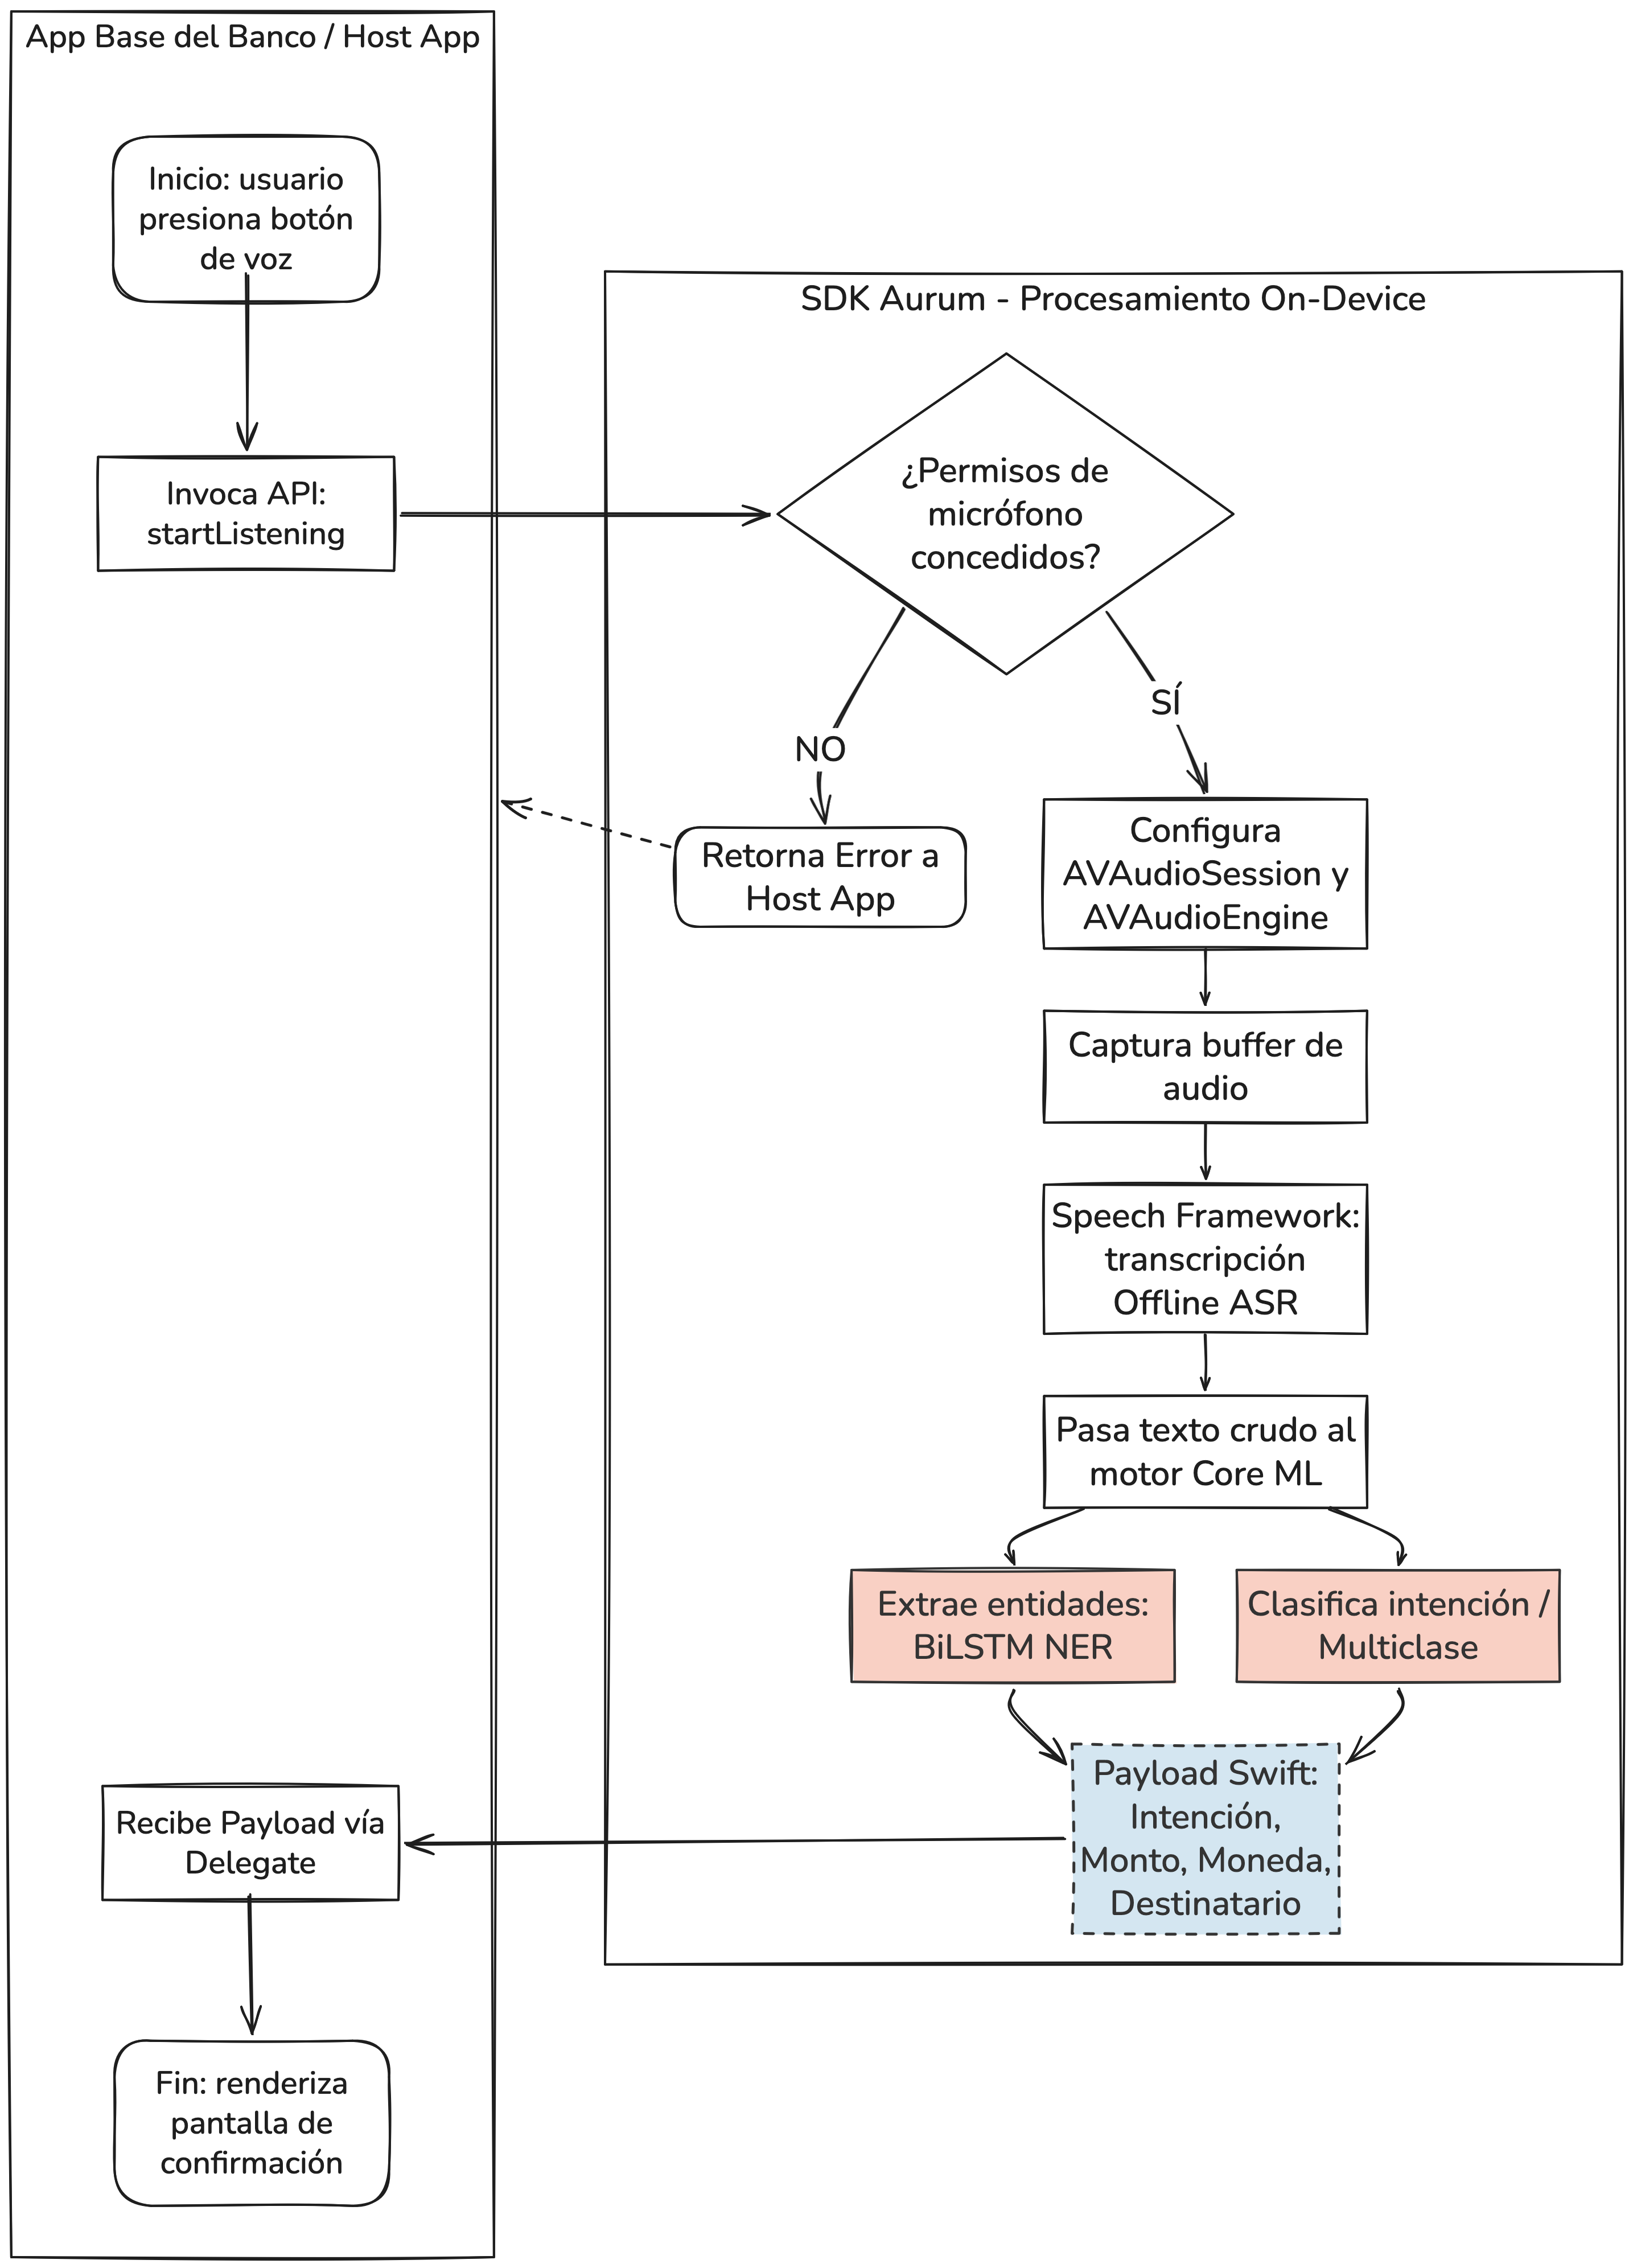
\includegraphics[width=1.0\textwidth]{./Figures/diagrama-flujo-aurum.png}
 \vspace{0.5cm} 
\caption{Diagrama de flujo de Aurum.}
\label{fig:diagAurum}
\end{figure}






